\section{Sample Use-Case}

\begin{figure}
\centering
  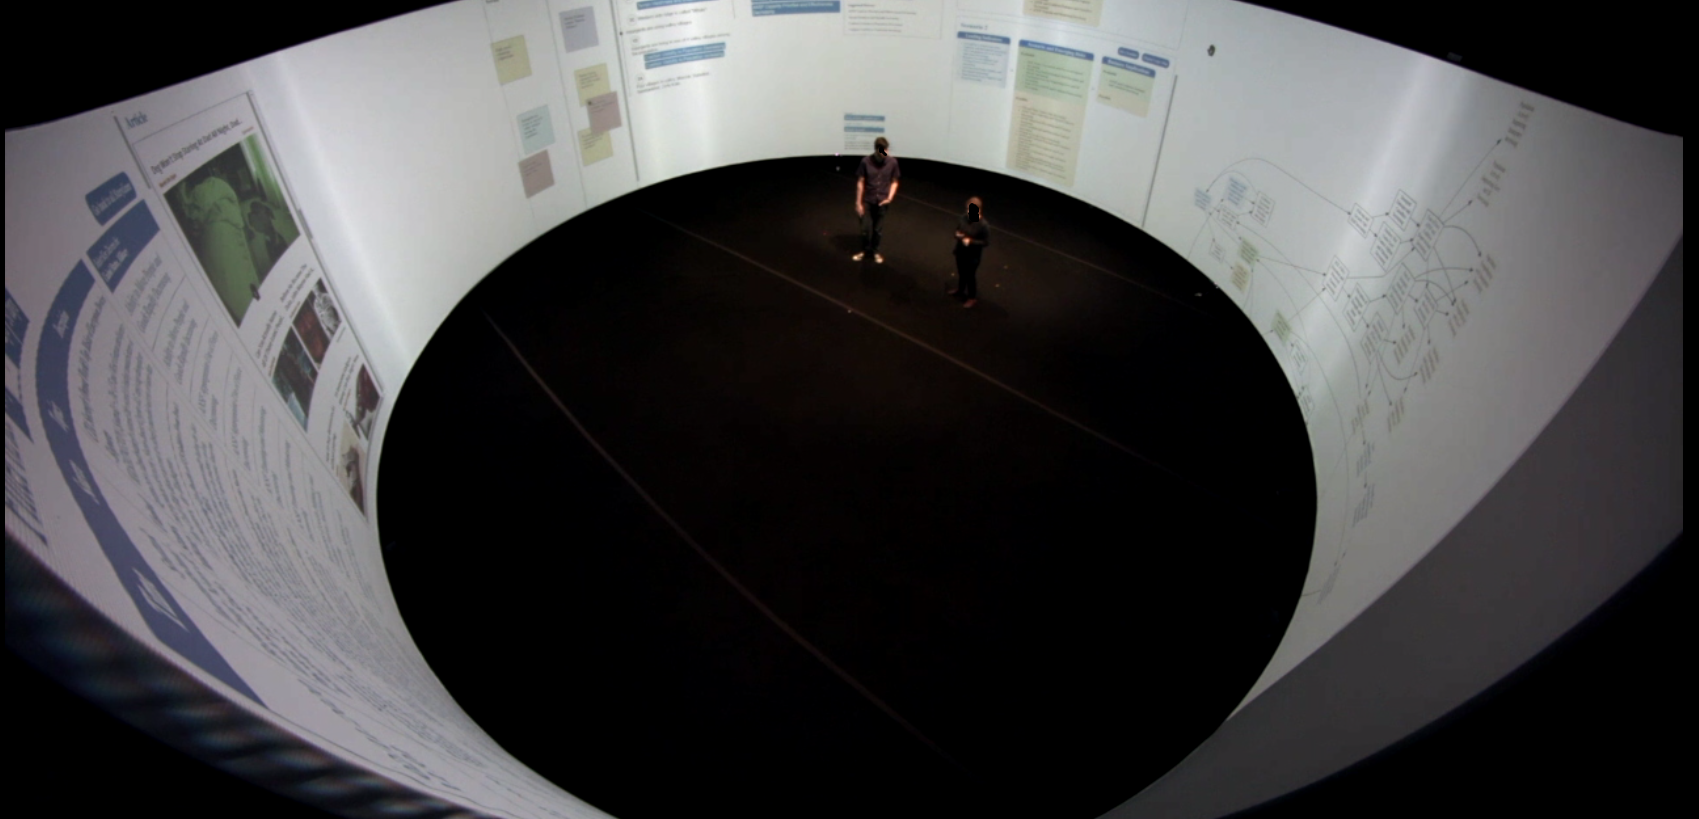
\includegraphics[width=0.8\columnwidth]{chapters/04_muifold/figures/demo_360.png}
  \caption{Overhead view of our use-case in the panoramic environment.}
  \label{fig:application_usecase}
\end{figure}

To demonstrate the effectiveness of our design, we created a sample
use-case centered around intelligence analysis, which brought together
multiple different applications into a single work-flow displayed
on a large 360° panaromic display, as shown in Figure~\ref{fig:application_usecase}~\footnote{A video of this demo 
use-case can be viewed at \url{https://www.dropbox.com/s/iokjvh0j6845688/iui_anonymous.mp4?dl=0}.}.
In this use-case, intelligent analysts are given a host of tools
to help them look at important news, create notes and hypothesises,
and generate ``what-if'' scenarios based on specific drivers they 
think could happen. For example, if the news talks about on-going
terrorist attacks within the Middle East, a driver they may select
would be ``Weakening of US and Allied Forces''.
Each piece of the application was implemented within its own webview 
open on the display server, and
where some utilized their own specific mobile UI, some did not. Each webview is always available to each user, and that they sit side-by-side to each other. We
briefly describe the different open webviews below. 

\subsection{Storyline Viewer}

This webview is composed of two parts. The first part gives a list
of ``storylines'', which is a grouping of articles pertaining to some
topic, like ``US, Military'' or ``Iraq, Trump''. This list can be
scrolled through, and clicking on a storyline will open up the list
of articles that are contained within that storyline. Clicking on an
article will then cause this view to issue a REST call to the display
server asking it to display the article's URL on the screen. There is
then a button to go back to the list of storylines, and clicking on
any column will cause the list to sort based on that column, first
ascending and then clicking again will cause it to be descending.
Currently, only one column will be sorted at a time. There is no
custom UI for the mobile application for this webview, however does
support left clicking and scrolling through the generic interface.

\subsection{Article Viewer}

As mentioned above, the Article Viewer is triggered by clicking on a
set article within the storyline viewer. This then triggers the
article to be loaded into its own set webview. These articles
come from various news organizations, such as the BBC, Reuters, etc.,
which we have no control over, but are still totally usable via our
generic interface, principally with scrolling through the article as well
being able to clicking on hyperlinks on the page to follow them.

\begin{figure}
\centering
    \hfill
    \subfigure[Storyline Viewer]{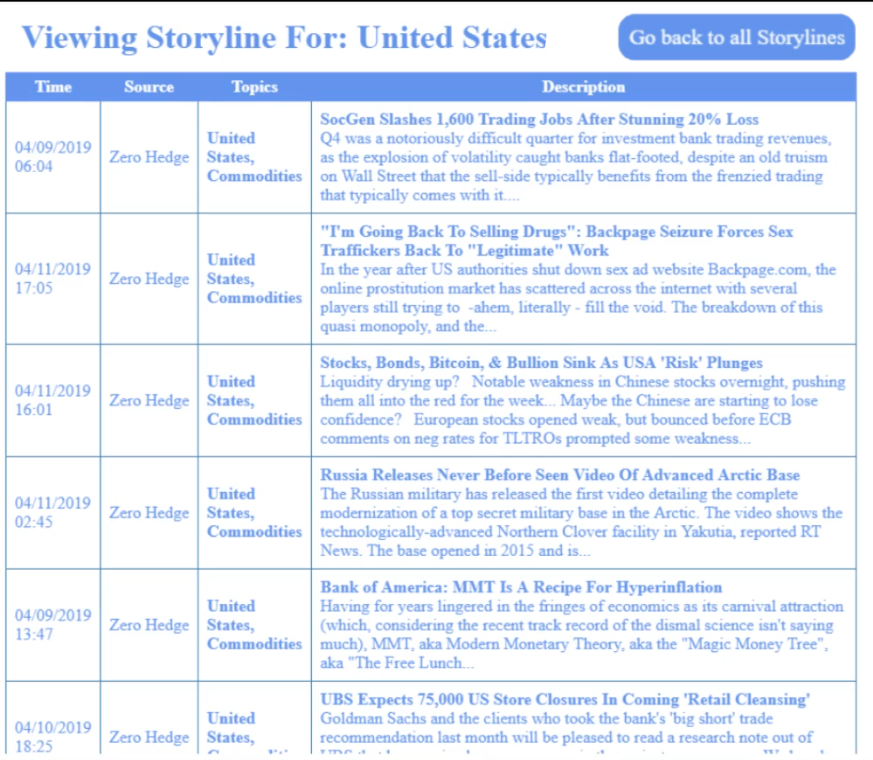
\includegraphics[width=0.3\columnwidth]{chapters/04_muifold/figures/storyline_viewer.png}}
    \hfill
    \subfigure[Article Viewer]{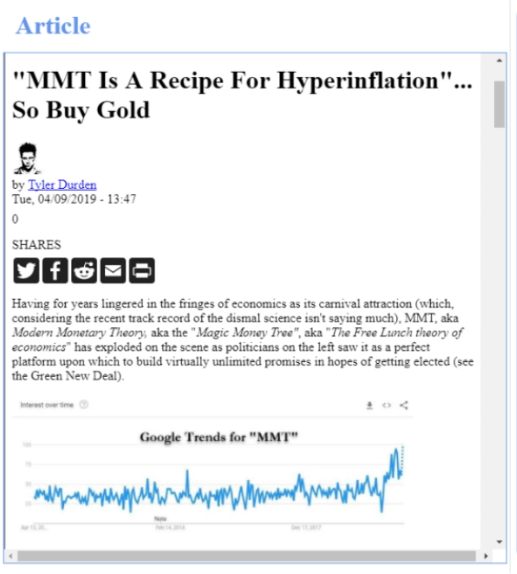
\includegraphics[width=0.25\columnwidth]{chapters/04_muifold/figures/article_viewer.png}}
    \hfill
    \\
    \hfill
    \subfigure[Scenario Generation Tool]{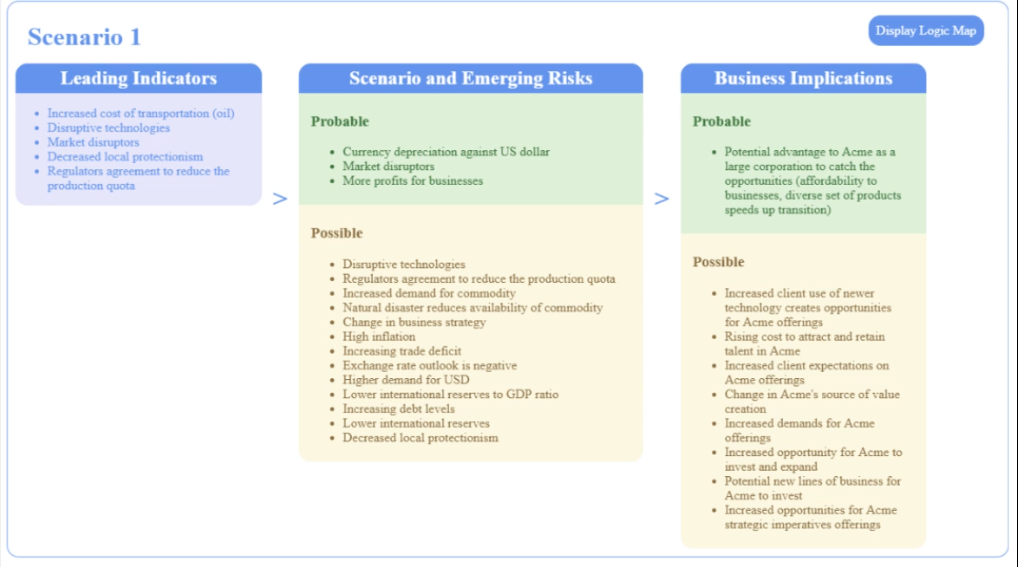
\includegraphics[width=0.4\columnwidth]{chapters/04_muifold/figures/scenario_planner.png}}
    \hfill
    \subfigure[Generated Scenario  Logic Map]{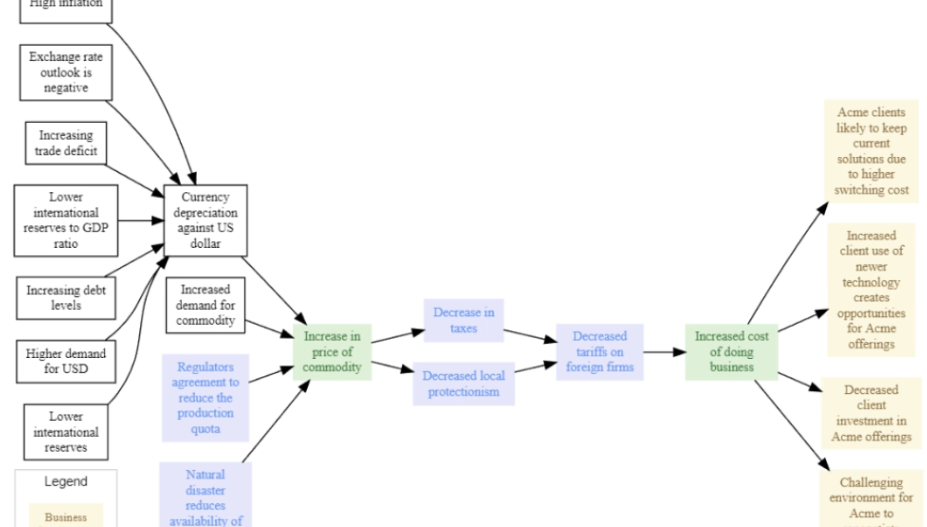
\includegraphics[width=0.4\columnwidth]{chapters/04_muifold/figures/scenario_planner_map.png}}
    \hfill
  \caption{Screenshots of different applications within the analyst use-case as shown on the large display.}
  \label{fig:application_specific_ui}
\end{figure}

\subsection{Sticky Notes}

The webview containing the sticky note application is usable only
through a custom UI, triggered once a user moves their cursor
over the webveiw and clicks the button at the bottom of the generic
UI. They are then greeted with a screen allowing them to turn on / off
the cursor, when they move the their cursor over a note, they can
grab a note, create a note, and place notes currently loaded on the
phone. Figure \ref{fig:application_specific_ui} gives a view of the
UI when a note is current being edited before being placed onto the
display. To handle interactions of notes between the phone and
webview, a WebSocket is opened specific to this application when
it is loaded on the client device. Once the client is finished with
this view, the WebSocket is closed.

\subsection{Prediction Creation Tool}

This webview contains predictions that are created by the analysts. Within our
environment, we provide space to create two hypothesises and to compare them
side-by-side. To utilize the tool, the analyst uses MUIFOLD to click on the
service on the large display. This opens an interface onto their phone where
they may write down the central prediction and then add as many minor supporting
predictions as they want. Under each supporting prediction, the user can then select
as many pieces of supporting evidence as they want, where each piece of evidence is
pulled from the sticky note application. The tool is shown in Figure~\ref{fig:prediction_ui}.

\subsection{Key Driver Selection Tool}

Key drivers are concepts of a scenario under analysis.
This tool provides usability in both the generic UI and also an
application specific UI for the client. Within the generic UI, a user
can left click on any previously selected driver to remove it
from the set under examination. Additionally, there is a dropdown
they can click to look at a list of all available drivers in the
system. This is shown in Figure ~\ref{fig:key_driver_tool}.
Alternatively, you can open an application specific UI on the client
which surfaces additional information, such as recently previously
selected drivers, drivers selected for previous scenarios, etc. that
would be not possible to display on the large display due to space
concerns.

\begin{figure}
\centering
    \hfill
    \subfigure[]{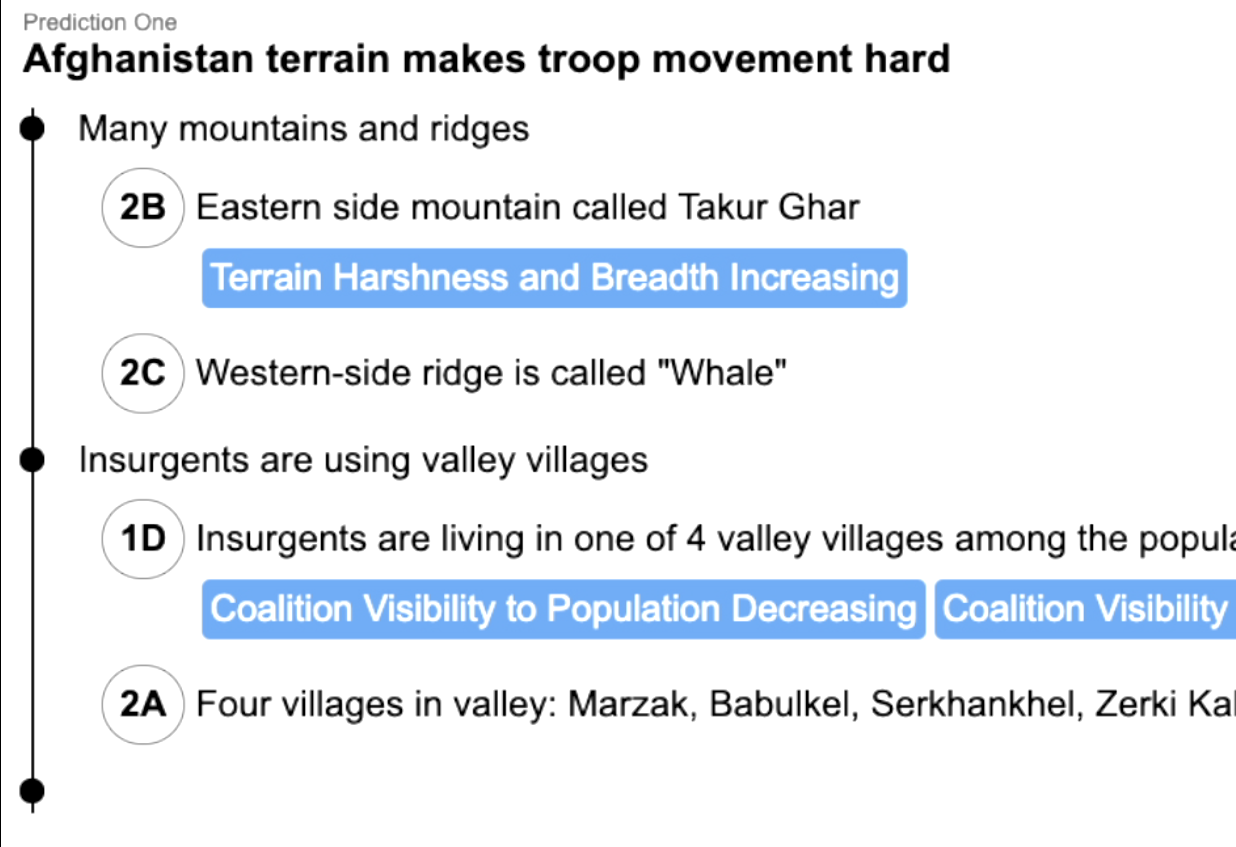
\includegraphics[width=0.5\columnwidth]{chapters/04_muifold/figures/hypthosis_generator.png}}
    \hfill
    \subfigure[]{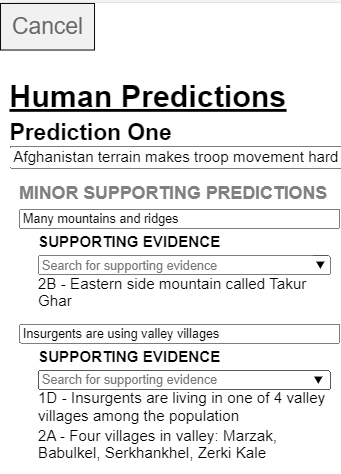
\includegraphics[width=0.25\columnwidth]{chapters/04_muifold/figures/hypthosis_muifold.png}}
    \hfill
  \caption{Screenshots of a) the hypothesis generation tool on the large display and b) its MUIFOLD interface.}
  \label{fig:prediction_ui}
\end{figure}

%\begin{figure}
%\centering
%  \includegraphics[width=0.4\columnwidth]{figures/mobile_ui_dropdown}
%  \caption{Generic UI with open dropdown.}
%  \label{fig:mobile_ui_dropdown}
%\end{figure}

\subsection{Scenario Generation}

After selecting drivers, a scenario is generated with a logic
map displayed using D3 and Graphviz, where showing the connections
between potential drivers that might have triggered or be triggered
by the selected drivers. Here, attempting to use the scroll detects
that the page itself cannot be scrolled, rather it can pan the D3
canvas, and so does that. Left clicking on a node in the graph
will trigger an event that either selects or deselects a driver. The
mobile specific UI here just mirrors down the graph to the personal
device, so a user can interact with it on their own. However, they can
lock the view of their personal device to that of the large display,
such that panning or zooming on the personal device will commit a
similar action on the large display. Communication here is done
through a websocket between the client and webview D3 instance,
where the zoom and pan coordinates are passed between the two, using
a fluid design for showing the content that fits the screen
real estate.

\begin{figure}
\centering
    \hfill
    \subfigure[]{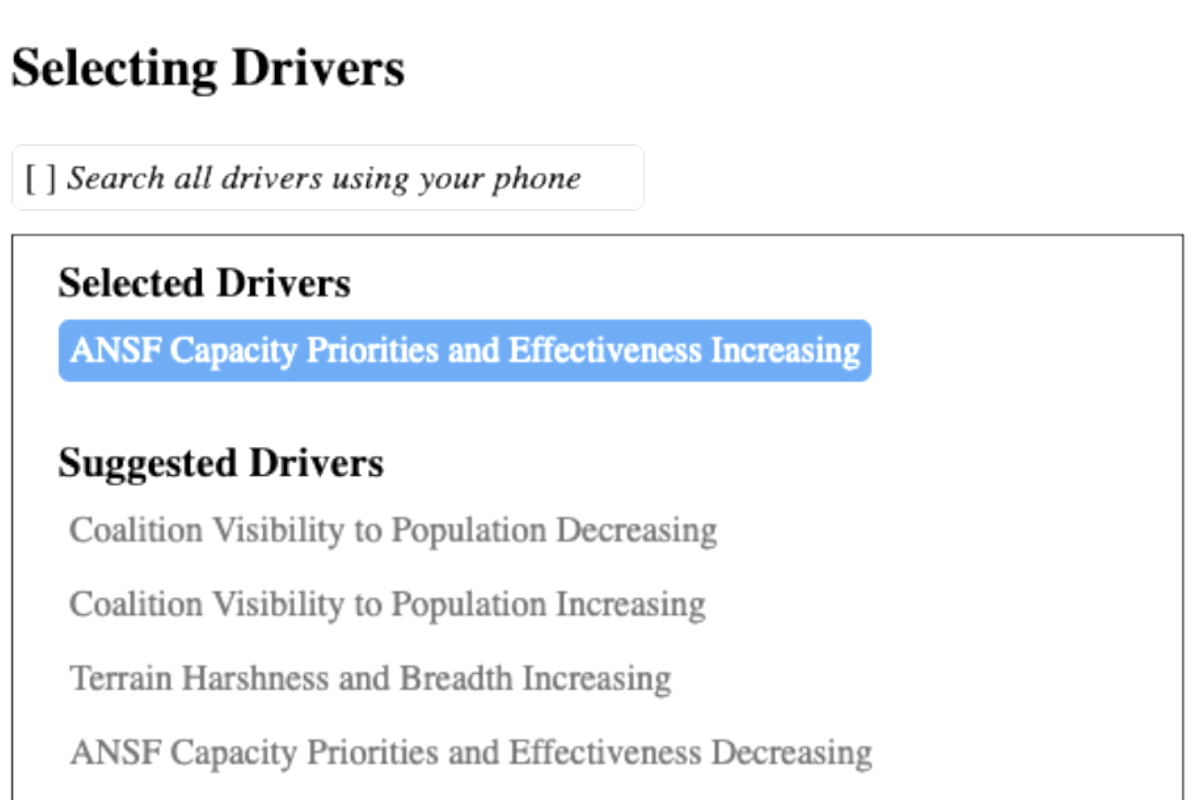
\includegraphics[width=0.5\columnwidth]{chapters/04_muifold/figures/driver_select_screen.png}}
    \hfill
    \subfigure[]{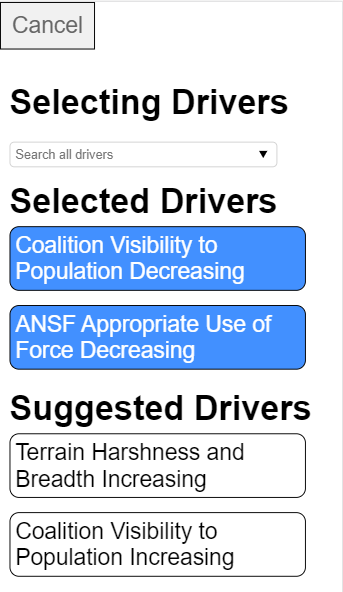
\includegraphics[width=0.25\columnwidth]{chapters/04_muifold/figures/driver_select_muifold.png}}
    \hfill
  \caption{Screenshots of a) the driver selection tool on the large display and b) its MUIFOLD interface.}
  \label{fig:key_driver_tool}
\end{figure}